% =====================================================================
%  cloud_intro.tex
% =====================================================================
\chapter{Cloud architecture}
\label{ch:overview}

This document describes how the functional architecture can be deployed on a cloud
infrastructure. During this phase, the architecture is designed without referring
to any specific cloud provider or technology, as these choices will be made during
the implementation phase.

\Cref{fig:architecture} shows the logical structure of the cloud architecture.
The circles placed one on top of another represent services running in multiple
instances. The red arrows show the prediction path, which is the only flow that
must meet the one-second response time requirement.

\begin{figure}[H]
\centering
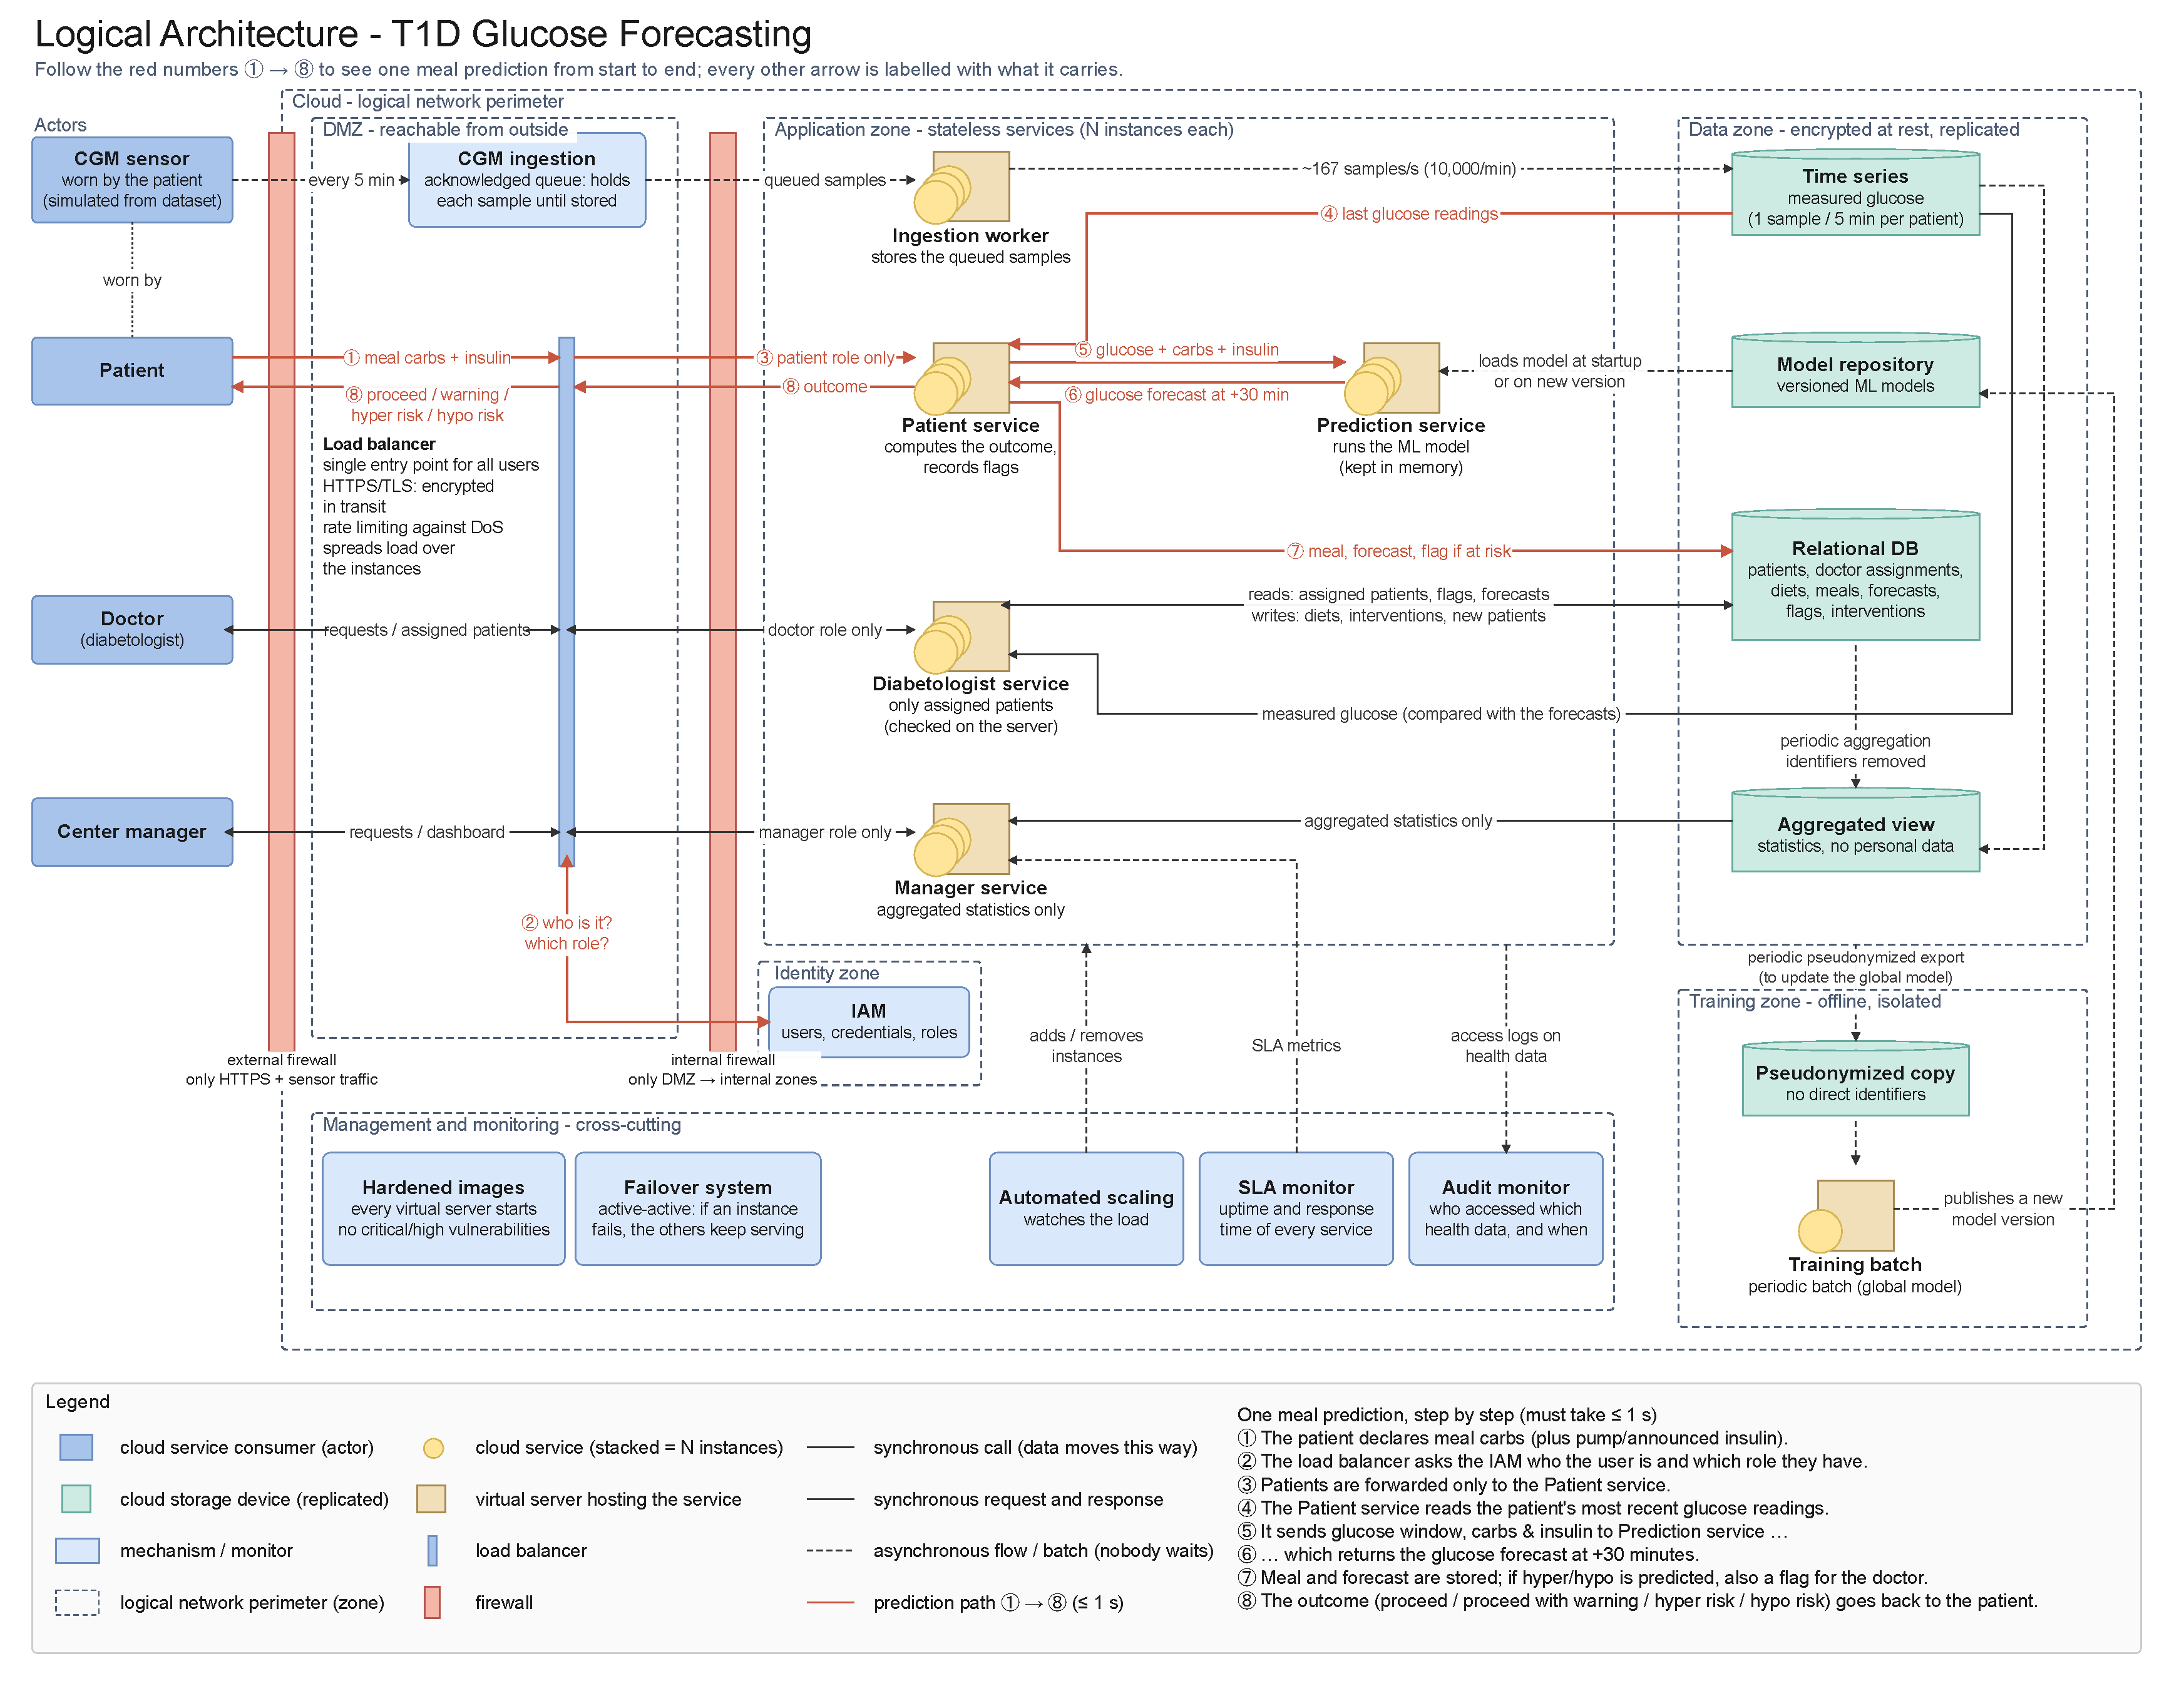
\includegraphics[width=\linewidth,height=0.92\textheight,keepaspectratio]{attach/arch.pdf}
\caption{Logical cloud architecture of the glucose forecasting service.}
\label{fig:architecture}
\end{figure}

The CGM sensor is represented as it would be in a real deployment: a separate
device worn by the patient that sends a new glucose sample every five minutes.
Since this project does not include a physical sensor, its behavior is simulated
by reading the samples from the dataset.

\section{Network zones}
\label{sec:zones}

The system is deployed within a logical network perimeter, which is further divided into separate zones, each one with its own perimeter (\cref{tab:zones}). 
Traffic is controlled by two
firewalls: the external firewall allows only HTTPS and sensor traffic to reach
the DMZ, while the internal firewall controls the traffic from the DMZ to the
internal zones, allowing only the connections required by the system.

\begin{table}[H]
\centering
\small
\rowcolors{2}{white}{softgrey}
\begin{tabularx}{\linewidth}{>{\raggedright\arraybackslash}p{3.4cm} Y >{\raggedright\arraybackslash}p{3.6cm}}
\toprule
\rowcolor{accent}
\tablehead{Zone} & \tablehead{Content} & \tablehead{Reachable from} \\
\midrule
DMZ                       & load balancer, CGM ingestion queue
                          & Internet, through the external firewall \\
Identity                  & IAM
                          & load balancer only \\
Application               & stateless services and ingestion worker
                          & DMZ, through the internal firewall \\
Data                      & encrypted and replicated storage devices
                          & application zone \\
Training                  & pseudonymized copy, training batch
                          & nobody (receives exports, publishes models) \\
Management and monitoring & hardened images, failover, scaling, SLA and
                            audit monitors
                          & administrators \\
\bottomrule
\end{tabularx}
\caption{Network zones of the architecture.}
\label{tab:zones}
\end{table}


The IAM is placed in a separate zone because it stores the credentials of all
users: even if an attacker manages to compromise a component in the
DMZ or the application zone, the IAM cannot be accessed directly from there.


The training zone is also kept isolated. This is because model training is an intensive task, has no strict timing requirements and does not require
access to the patients' identities.